\documentclass{article}
\usepackage{graphicx}
\usepackage{geometry}
\usepackage{amsmath}
\usepackage[numbers,sort&compress]{natbib} 
\usepackage{float}
\usepackage{bm}
\usepackage{fontspec}
\usepackage{amsfonts}
\usepackage{booktabs}
% \setmainfont{Calibri} %字体
% \usepackage[UTF8]{ctex} %中文包
\usepackage{xcolor}
\geometry{a4paper,scale=0.8}
\title{Machine learning number of Dirac cones with neural networks}
\author{JunAng Wang}
\begin{document}
\maketitle
Recent, machine learning has emerged as a powerful tool in various scientific disciplines. Particularly, some researchers have begun to utilize  machine leaning to solve many-body physics problems in the recent year \cite{carleo2019machine,carrasquilla2020machine,johnston2022perspective}, e.g. classifying phases\cite{carrasquilla2017machine,wang2016discovering,tanaka2017detection,zhang2018machine}, representing many-body wave function\cite{carleo2017solving,sharir2020deep}, speeding up many-body simulations\cite{chen2018symmetry,wu2019solving,nagai2017self,liu2017self} et al.   In our previous work titled " Topological Quantization of Superfluid Stiffness in Dirac Materials"\cite{wang2022topological}, we demonstrated the mechanism of the quantization of the superfluid stiffness in Dirac materials. Our findings revealed that the superfluid stiffness in Dirac materials remains quantized as long as the number of Berry monopoles is conserved in the synthetic space. Specifically, in the case of charge-neutral and Zeeman field neutral conditions, the superfluid stiffness($ D_{\textrm{total}}  $) is equal to $  \frac{\Delta}{\pi}  $  per cone (we will derive a more general $ D_{\textrm{total}} $ later ). Therefore the quantity of superfluid stiffness is determined by the number of Dirac cones present. This raises a intriguing question: can we establish a mapping from the value of superfluid stiffness to the number of Dirac cones? Such a mapping would have practical implication allowing experimentalists to determine the number of Dirac cones by measuring the superfluid stiffness of real materials, like graphene.

In this note, we aim to address above question through a supervised machine learning approach. We train our neural network by feeding superfluid stiffness data obtained from the Dirac model that may encompass higher order Dirac cones, enabling it to predict the Hamiltonian's total absolute vorticity. The total absolute vorticity is equal to the number of Dirac cones times their corresponding order.  After fully training our network, we test our model's performance using superfluid stiffness data for graphene which is a 2D material. Our model achieve a high accuracy, which validates the effectiveness of our method.

\section{Dirac model and higher order band touching points}
In this section, we will introduce the Dirac model and derive the corresponding superfluid stiffness. It's important to note that we utilize Dirac model's superfluid stiffness as input for our neural network during training process.

The Hamiltonian of the Dirac model in momentum space can be written as 
\begin{align}
    \hat{h} &= \left(a k_x + ib k_y\right)^n \hat{\sigma}_+ + \left(a k_x - ib k_y\right)^n \hat{\sigma}_- + \mu_0 \\
            &= |\widetilde{k}|^n \cos(n \theta) \hat{\sigma}_x - |\widetilde{k}|^n \sin(n \theta) \hat{\sigma}_y + \mu_0\\
            &= |\widetilde{k}|^n e^{in \theta \hat{\sigma}_z}\hat{\sigma}_x + \mu_0,  
\end{align}
where $ \mu $ is chemical potential, $ n $ is a positive integer, $ \hat{\sigma} $ denote Pauli matrices in sub-lattice space, $ |\widetilde{k}|= \sqrt{(a k_x)^2 + (b k_y)^2 }   $ and $ \tan(n \theta) = \frac{(ak_x-ibk_y)^n}{(ak_x+ibk_y)^n} $. The eigen-vector of the Hamiltonian is read as 
\begin{align}
    |u_\pm\rangle = \frac{1}{\sqrt{2} } \left(\begin{array}{c}
         1 \\
         \pm e^{-in \theta} \\
    \end{array}\right),
\end{align}
whose corresponding eigen-value is presented as $ \epsilon_{\pm} = \pm |\widetilde{k}|^n + \mu_0   $. 

Now let's consider that superconductivity is introduced into the system. The super current flow in the direction of gradient of superconducting phase $ \phi $ proportional to superfluid stiffness, such as $ J_{i}=D_{ij}\nabla_i \phi$, where superfluid stiffness $ D $ is a symmetric matrix
\begin{align}
    D & = \left(\begin{array}{cc}
        D_{xx}  & D_{xy}    \\
        D_{yx}  & D_{yy}   \\
    \end{array}\right)
\end{align}
The element of superfluid stiffness can be read as:
\begin{align}
    D_{ij} = 2\Delta^2 \iint \frac{dk_x}{2\pi} \frac{dk_y}{2\pi} \sum_{\alpha,\beta=\pm} \frac{\langle u_{\alpha}|\partial_{i} \hat{h}|u_{\beta}\rangle\langle u_{\beta}|\partial_{j} \hat{h}|u_{\alpha}\rangle}{E_\alpha^2 - E_\beta^2} \left(\frac{f(E_\beta)}{E_\beta} - \frac{f(E_\alpha)}{E_\alpha} \right),\label{eq:SS}
\end{align} 
where $ i,j \in \{x,y\} $, $ f(E) = \Theta(B+E)-\Theta(B-E)=\Theta(E-\left\vert B \right\vert ) $ and $ E_\pm = \sqrt{\epsilon_\pm^2 + \Delta^2}  $. Utilizing Eq. (\ref{eq:SS}), we immediately obtain the superfluid stiffness of the Dirac model,
\begin{align}
    D_{xx}  &=\frac{a}{b} (D_{\textrm{intra}} + D_{\textrm{inter}}),\\ \label{eq:Dxx }
    D_{yy}  &=\frac{b}{a} (D_{\textrm{intra}} + D_{\textrm{inter}}),\\ \label{eq:Dyy }
    D_{xy} &= D_{yx} = 0,
\end{align}
where
\begin{align*}
    D_{\textrm{intra}} &=  n \frac{\sqrt{\mu_0^2+\Delta^2}}{2\pi}\Bigg\{ \Theta(|\Delta|-|B|)+\Theta(|B|-|\Delta|)\Theta(\sqrt{\mu_0^2+\Delta^2}-|B|) \bigg[1-\frac{|\mu_0|}{\sqrt{\mu_0^2+\Delta^2}}\frac{|B|}{\sqrt{B^2-\Delta^2}}\bigg]\Bigg\},\\
    D_{\textrm{inter}} &= \frac{n}{|\mu_0|}\frac{\Delta^2}{2\pi} \Bigg\{ \Theta(|\Delta|-|B|)\ln(\frac{\sqrt{\mu_0^2+\Delta^2}+|\mu_0|}{|\Delta|})+\Theta(|B|-|\Delta|)\Theta(\sqrt{\mu_0^2+\Delta^2}-|B|)\ln(\frac{\sqrt{\mu_0^2+\Delta^2}+|\mu_0|}{\sqrt{B^2-\Delta^2}+|B|}) \Bigg\}.    
\end{align*}
when $\mu_0 \to 0$, $D_{\textrm{inter}}=n\frac{|\Delta|}{2\pi}\Theta(|\Delta|-|B|) $. For zero Zeeman field and chemical potential, $ D_{xx}=D_{yy} = n \frac{\left\vert \Delta \right\vert}{\pi}     $ which aligns in our initial statement. 

In  order to eliminate the effect of anisotropy, we are interested at the determinant of superfluid stiffness 
\begin{align}
    \left\vert D \right\vert &= D_{xx}D_{yy} - D{xy}D{yx}\label{eq:D}\\
                             &= D_{\textrm{total}}^2, 
\end{align}
which does not include $ a,b $.  Here $ D_{\textrm{total}} = D_{\textrm{intra}} + D_{\textrm{inter}} $. By considering the determinant, we can effectively capture the overall behavior and characteristics of the superfluid stiffness, while cancels the influence of the inherent anisotropy present in the system. 
It is worth to notice that $ |D|=D_{\textrm{total}}^2  $ appears because of $ D_{xy}= D_{yz} = 0   $ in Dirac model, for more general case we need to calculate  Eq. (\ref{eq:D}). For convenience, in the following discussion we set $ \Delta = 1 $. Figure. (\ref{fig: Deter_D_3D}) illuminates the amplitude of $ |D| $ with $ \mu_0 $ and $ B $ varying in the range of $ \left(-3,3\right) $. Notably,one may observe that $ |D| $ changes discontinuously at $ |B| = \Delta $, specifically when $ \mu_0=0 $ $ |D| $ experiences an abrupt drop $ \frac{1}{\pi^2} $ (see inset figure). This discontinuity may serves as an crucial signal in identifying the so called total absolute vorticity. 

\begin{figure}[H]
    \centering
    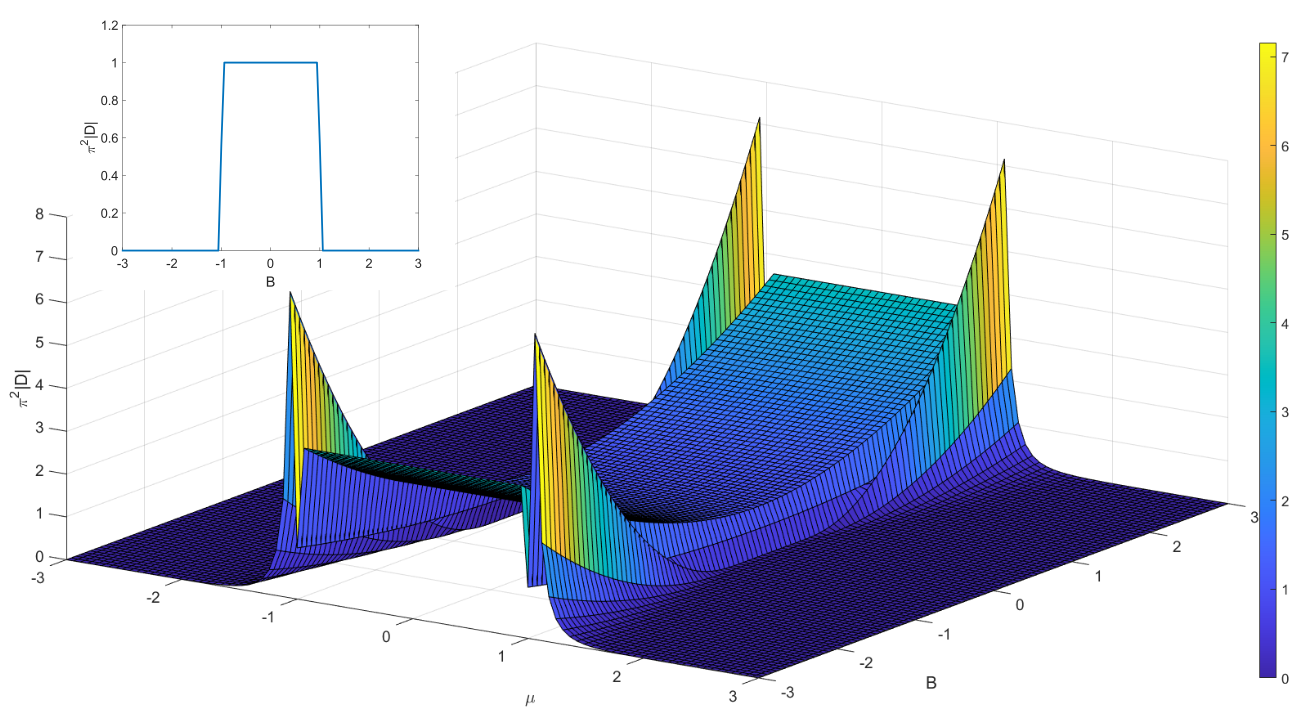
\includegraphics[width=0.8\textwidth]{matlab code/D_deter_3D_hybrid.pdf}
    \caption{Amplitude of $ |D| $ with $ mu_0 $ and $ B $ varying in the range of $ \left(-3,3\right) $. Inset figure shows variation of $ |D| $ with $ B $ varying and $ \mu_0 =0 $. }
    \label{fig: Deter_D_3D}
\end{figure}

\subsection{Total absolute vorticity}
The total absolute vorticity is equal to the number of Dirac cones times their corresponding order, which is our neural network's main prediction. One can rewrite above Dirac model Hamiltonian as a vector form 
\begin{align}
    \hat{h} &= \mathbf{H} \cdot \bm{\sigma},
\end{align}
where $ \mathbf{H}= \left(|\widetilde{k}|^n \cos(n \theta),|\widetilde{k}|^n \sin(n \theta) \right) $. The angle of vector $ \mathbf{H} $ is denoted by $ \phi = \arctan(-\tan(n \theta)) = -n \theta $. The total absolute vorticity is written as 
\begin{align}
    w &= \frac{1}{2\pi}\left\vert \oint d \phi  \right\vert =  n. 
\end{align}

\section{Parabolic model}
In previous section, we compute the contribution of a single Dirac cone to superfluid stiffness. In this section, we study the contribution of a trivial crossing point of the Fermi level to the superfluid stiffness. Without loss generality, we study the parabolic model whose Hamiltonian can be written as 
\begin{align}
    \hat{h}_{\textrm{p}} &= \left[(a k_x)^2 + (b k_y)^2\right] \hat{\sigma}_x + \mu_0 
\end{align}
whose eigen-vectors are 
\begin{align}
    u^{\textrm{p}} _\pm &= \left(\begin{array}{c}
         1 \\
         \pm 1 \\
    \end{array}\right)
\end{align}
corresponds to eigen-value $\epsilon^{\textrm{p}}_\pm =  \pm |\widetilde{k}|^2 + \mu_0  $. Applying Eq. (\ref{eq:SS}), the contribution to the superfluid stiffness is 
\begin{align}
    D^{\textrm{p}} _{xx} &= \frac{a}{b}D_{\textrm{intra}}, \\   
    D^{\textrm{p}} _{yy} &= \frac{b}{a}D_{\textrm{intra}}, \\   
    D^{\textrm{p}} _{xy} &= D^{\textrm{p}}_{yx} =0. 
\end{align}
For trivial case, the interband part of superfluid stiffness is equal to zero. 

Since the parabolic model's Hamiltonian only have contribution to $ \hat{\sigma}_x $, then the corresponding vorticity is equal to zero. 

\section{Training data set}
Before constructing the input data set, it's important to emphasize the primary objective of our neural network. Our neural network aims to predict two key aspects: firstly, whether the crossing point of the Fermi level corresponds to a Dirac cone. Secondly, the number of Dirac cones within a small window as the parameters $ B $ and $ \mu_0 $ vary.



\begin{figure}[H]
    \centering
    \includegraphics[width=1\textwidth]{Training Data.pdf}
    \caption{Training data set example. The first row illustrates the determinant of superfluid stiffness for a parabolic model with $ \mu_0 $ varying in the range of $ \left(-3,3\right) $, $  \mu_{\textrm{off}} = B_{\textrm{off}} = 2$  . The second row represents the determinant for a Dirac model($ n=1 $) where $ \mu_0 $ varies in the same range. The corresponding vorticity is shown above the matrix.}
    \label{fig: Training Data}
\end{figure}
\section{Neural network}
In this note, we have chosen the convolutional neural network(CNN)\cite{lecun1998gradient,krizhevsky2012imagenet,goodfellow2016deep} to classify the total absolute vorticity due to the crucial information concentrated along the $ B=\Delta $ edge. The convolutional neural network is particularly effective at detecting and learning oriented edges, making it well suited for capturing the relevant features in our data . The neural network work flow and the structure is shown in Fig. (\ref{fig: Neural network}). 

The architecture of neural network structure is a simple and standard CNN classifier. One input the determinant of superfluid stiffness to the neural network which output the total absolute vorticity. The neural network encompass two convolutional layers with 32 channels of kernel size $ 3 \times 3 $ and 2 channels of kernel size $ 3 \times 3 $, followed by two fully connected layers with the first one containing 1024 neurons and the second 512 neurons. At last, the neural network output the scores for 8 categories. The first 7 categories identify the total absolute vorticity from $ 0 $ to $ 6 $ and the last one match the total absolute vorticity above $ 6 $. By applying softmax function to normalize and convert the scores to possibilities. Consequently, the neural network provide the most probable total absolute vorticity as its output. All the hidden layers in the network are equipped with the rectified linear units(ReLU) $ f(x) =\max\{0,x\} $ as activation function and the ouput layer utilizes linear activation $ f(x)=x $. The learning rate and regularization strength is set to $ 10^{-3}  $ and $ 0 $, respectively.
\begin{figure}[H]
    \centering
    \includegraphics[width=1\textwidth]{Neural network.pdf}
    \caption{Schematic of the machine learning workflow and the structure of the convolutional neural network.}
    \label{fig: Neural network}
\end{figure}

We generate Dirac model data set by using the approach discussed earlier. We split the Dirac and parabolic model data set into 2 part, $ 4 \times 10^3 $ determinant samples with the total absolute vorticity $ w \in \left(0,7\right) $, randomly choose $ 90\% $ of them for training data set and the remainder as (i) the first validation data set which was not used during training process; $ 10^3 $ samples with the total absolute vorticity $ w \in \left(8,9\right) $ (ii) as the second validation data set whose vorticity is unseen in training process. And set $ mu_0 $ ranges in $ \left(-5,5\right) $. During training, our neural network minimize the cross-entropy loss\cite{hinton1995wake} to learn the patterns in the data by the adam optimizer\cite{kingma2014adam}. 

After training, we evaluated the performance of our model by validation data set and achieved an accuracy of $ 99.60\% $ for data (i) and $ 99.15 \% $ for data (ii). This high accuracy indicates that our neural network effectively identify and classify the total absolute vorticity of ideal Dirac model. In order to guarantee our method is suitable for real materials, in the following we evaluate our model by graphene data. The network construction and training were performed using  PyTorch platform\cite{paszke2019pytorch} .


\section{Graphene model}
In this note, we validate our neural network by testing a real material model, the graphene model. Graphene is made out of carbon atoms arranged in hexagon structure which can be viewed as two atoms per unit cell. Thus graphene possesses the so called sublattice symmetry (chiral symmetry). The Hamiltonian of Graphene in momentum space can be written as 
\begin{align}
    \hat{h}_{\textrm{g}} = &-t \left[\cos(\frac{1}{2}k_x + \frac{\sqrt{3}}{2} k_y )+ \cos(\frac{1}{2}k_x - \frac{\sqrt{3}}{2} k_{y}  )+ \cos(-k_x)\right] \hat{\sigma}_x \nonumber\\
    &-t \left[\sin(\frac{1}{2}k_x + \frac{\sqrt{3}}{2} k_y )+ \sin(\frac{1}{2}k_x - \frac{\sqrt{3}}{2} k_y )+ \sin(-k_x)\right] \hat{\sigma}_y+\mu,
\end{align}
where $ t \approx 2.8eV $ is hopping amplitude. $ \hat{\sigma} $ are Pauli matrices acting on sub-lattice space.

The eigen-energy have formula $ \epsilon^{\textrm{g}}_\pm = \pm t \sqrt{3+2 \cos(\sqrt{3} k_y )+4 \cos(\frac{\sqrt{3}}{2}k_y ) \cos(\frac{3}{2}k_x)} + \mu  $ and its corresponding eigen-vector can be read as 
\begin{align}
    u^{\textrm{g}}_\pm = \frac{1}{\sqrt{2} } \left(\begin{array}{c}
         1 \\
         \pm i e^{i \theta_{\textrm{g}} } \\
    \end{array}\right),
\end{align}
where
\begin{align}
    \tan(\theta_{\textrm{g}} ) &= \frac{\sin(\frac{1}{2}k_x + \frac{\sqrt{3}}{2} k_y )+ \sin(\frac{1}{2}k_x - \frac{\sqrt{3}}{2} k_y )+ \sin(-k_x)}{\cos(\frac{1}{2}k_x + \frac{\sqrt{3}}{2} k_y )+ \cos(\frac{1}{2}k_x - \frac{\sqrt{3}}{2} k_{y}  )+ \cos(-k_x)} 
\end{align}
Applying Eq. (\ref{eq:SS}), one obtain the determinant of graphene's superfluid stiffness. 

\subsection{Total absolute vorticity of graphene}
Since the hopping amplitude is much larger than the induced superconductivity in graphene $ \Delta \approx 1meV $, the Hamiltonian can be approximately described by two Dirac cones 
\begin{align}
    \hat{h}_{\textrm{g}} &\approx   v_{F} \left( q_x \hat{\sigma}_x + q_y \hat{\rho}_z \hat{\sigma}_y \right) + \mu_0,
\end{align}
where $ \mathbf{q} $ is the momentum measured relatively to the Dirac points, $ v_F $ is the Fermi velocity, given by $ v_F = \frac{3}{2} t $, $ \hat{\rho} $ are Pauli matrices in valley space. 

The total absolute vorticity is the sum of absolute vorticity of two containing Dirac cones, i.e. $ w_{\textrm{g}} \approx 2  $. The determinant of graphene would be labeled as $ 2 $ if Dirac cones present within the defined window, else would be labeled as $ 0 $. By varying hopping amplitude and central chemical potential, one gather a set of test date.



\subsection{The performance of neural network}
(iii)We generate determinant samples from graphene with $ t \in \left(3000,4000\right) $ as test data set. Figure (\ref{fig:Acc_density_spectrum}) illustrates the performance of network plot versus the number of training samples. The green and blue dots depict the accuracy of the first (i) and the second (ii) validation data set, respectively, reaching an accuracy $ 99.60 \% $ and $ 99.16 \% $ with training on $ 3500 $ samples. Meanwhile the red dots represent the accuracy achieved on the (iii) graphene data, which attains an accuracy of $ 95.00 \% $. Notably, as the number of training data increases, the accuracies of all mentioned data improve indicating the beneficial impact of augmenting the training data size. The observation reflects the network's capability to enhance its predictive capability and as it learns from larger and more diverse training data. The test result is presented in Table (\ref{tab:Performance}). 

The sketch (Figure (\ref{fig:Acc_density_spectrum})(b)) shows the graphene spectrum in momentum space projecting on the $ k_y $ axis, where two Dirac points are located at the chemical potential $ \mu_0 = 0 $. The green and red boxes represent two examples of the previously discussed scanning windows concentrated at $ \mu_0 = 0 $ and $ \mu_{0} = 4.2 $, ranging in $ \left(\mu_0 - 2, \mu_0 + 2\right) $. The green box predicts the total absolute vorticity $ w $ to be equal to $ 2 $, while the red box predicts $ w = 0 $. The figure on the right-hand side demonstrates our network's performance in $ 15 $ energy bins. Our results achieve high accuracy of around $ 100 \% $, except for a drop to approximately $ 69 \% $ in the bins $ 1.67 < |\mu_0| < 2.33 $. The reason for the accuracy drop is that the Dirac points are located around the edge of the scanning window, leading to ambiguity and harmful impact on predictions

\begin{figure}[H]
    \centering
    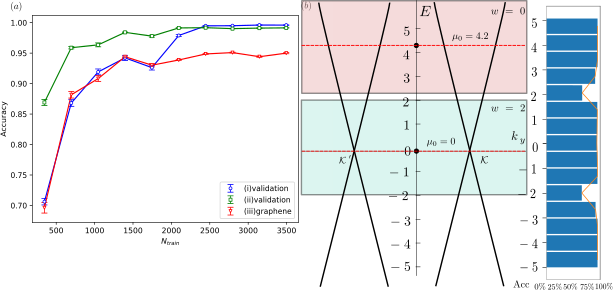
\includegraphics[width=1\textwidth]{Accuracy_density_spectrum.pdf}
    \caption{(a) The performance of the network versus the number of training samples. The green, blue and red dots represent the accuracy of the first (i) and the second (ii) validation data set and (iii) graphene data, respectively, reaching an accuracy $ 99.60 \% $, $ 99.16 \% $ and $ 95.00 \% $ with training on $ 3.5 \times 10^3 $ samples. One can obverse that the accuracies of all data sets increase with more training data. (b) Sketch of graphene spectrum in momentum space, projecting on $ k_y $ axis, with two Dirac points locate at $ \mu_0=0 $. The green and red box depict two examples of previous discussed scanning windows concentrated at $ \mu_0=0 $ and $ \mu_{0} = 4.2  $, range in $ \left(\mu_0 -2,\mu_0 +2\right) $. The green box predicts the total absolute vorticity $ w $ equal to $ 2 $ while the red box predicts $ w=0 $. The figure on the right hand side demonstrates the our network's performance in $ 15 $ energy bins, achieving high accuracy around $ 100 \% $, except for a drop to approximately $ 69 \% $ in the bins $ 1.67<|\mu_0|<2.33$. The accuracy drop is due to ambiguity caused by the proximity of the Dirac points to the edge of the scanning windows. }
    \label{fig:Acc_density_spectrum}
\end{figure}

\begin{table}[H]
    \centering
    \begin{tabular}{c|c|c|c}
        \toprule
             & Validation(i)  & Validation(ii) & Test(iii)   \\
        \midrule
        Accuracy     & 99.60\% & 99.15\% &  95.00\%  \\
        \bottomrule
    \end{tabular}
    \caption{Performance of the neural network training by $ N_{\textrm{trian}} = 3500  $ with respect to different validation and test data sets.}
    \label{tab:Performance}
\end{table}

\section{Chiral symmetry broken model}
In the real world, materials may or may not possess chiral symmetry.  To demonstrate the effectiveness of our neural network in broader applications, we evaluate it by a chiral symmetry broken model
\begin{align}
    \hat{h}_{\textrm{g}} = &-t \left[\cos(\frac{1}{2}k_x + \frac{\sqrt{3}}{2} k_y )+ \cos(\frac{1}{2}k_x - \frac{\sqrt{3}}{2} k_{y}  )+ \cos(-k_x)\right] \hat{\sigma}_x \nonumber\\
    &-t \left[\sin(\frac{1}{2}k_x + \frac{\sqrt{3}}{2} k_y )+ \sin(\frac{1}{2}k_x - \frac{\sqrt{3}}{2} k_y )+ \sin(-k_x)\right] \hat{\sigma}_y+\mu_0 + \textrm{Sign}(k_y)\delta \mu.
    \label{eq: Modified Graphene}
\end{align}
This model involves the graphene Hamiltonian, which is modified by a chemical potential $ \delta \mu $ depending on the sign of $ k_y $ in the first Brillouin zone. As a result, the two Dirac cones in the model are not longer aligned at the same energy level but shifted by $ \delta \mu $, the low energy effective model can be expressed as
\begin{align}
    \hat{h}_{\textrm{g}} &=   v_{F} \left( q_x \hat{\sigma}_x + q_y \hat{\rho}_z \hat{\sigma}_y \right) + \delta \mu \hat{\rho}_z + \mu_0.
\end{align}
\subsection{Train the network}
We utilize the previously discussed data set and compute the determinant superfluid stiffness of a Dirac model containing two Dirac points permuting in the full spectrum ($ |D_1 + D_2| $). For better comparison, we set the maximum vorticity of every individual Dirac point to $ \max(|D_1|) = \max(|D_2|) =  9 $ and the maximum of total vorticity of the full system is also set to $ \max(|D_1 + D_2|) = 9 $.  This approach allows us to generate a new data set with $ \mu_0 \in \left(-5,5\right) $, $ \delta \mu \in \left(-5,5\right) $, $ w \in \left(0,9\right) $ containing around a total of $ 5 \times 10^4 $ samples. We split the data set into 2 part: the first part include $ 4.5 \times 10^4 $ samples with $ w \in \left(0,7\right) $ and the second part contains $ 0.5 \times 10^4 $ samples with $ w \in \left(8,9\right) $ forming the unseen $ w $ validation data set (v). Moreover, $ 90 \% $ of the first part samples used as new training data set and the remainder forming (iv) the validation data set which remained unseen during training process. Additionally, we generate the determinant $ |D| $ for modified graphene model Eq. (\ref{eq: Modified Graphene}) as test data set (vi). Sketch (\ref{fig:Acc_density_spectrum_broken}(b)) depicts the modified graphene low energy effective spectrum, similarly to sketch (\ref{fig:Acc_density_spectrum}(b)) the system containing two Dirac cones however the cones shifted by chemical potential $ \delta \mu $. Three examples of scanning windows are shown in the sketch, unlike only predicting $ w=0 $ and $ w=2 $ in sketch (\ref{fig:Acc_density_spectrum}(b)), sketch (\ref{fig:Acc_density_spectrum_broken}) predict cases $ w=1 $ due to nonzero $ \delta \mu $ ,seen in the blue box where $ \mu_0=-2.2 $.  Additionally, the accuracy density plot illuminates the accuracy remain relative high expect the ambiguous situation discussed earlier. 

After training our network on the training data, we validate the performance of our network by using data (iv), (v) and (vi). We achieve an accuracy of $ 98.26 \% $ for (iv), $ 98.18 \% $ for (v) and $ 90.54\% $ for (vi). The high accuracy demonstrate the effectiveness of our method for chiral symmetry broken material, further proving the versatility and robustness of our approach. Figure (\ref{fig:Acc_density_spectrum_broken}(a)) depicts the performance of the network to chiral symmetric broken two-Dirac-points systems versus the training scale. The accuracies improve as the training scale increasing.    

\begin{figure}[H]
    \centering
    \includegraphics[width=1\textwidth]{Accuracy_density_spectrum_broken_v2.pdf}
    \caption{(a) The performance of the network to chiral symmetric broken systems versus the number of training samples. The green, blue and red dots represent the accuracy of the first (iv) and the second (v) validation data set and (vi) modified graphene data, respectively, reaching an accuracy $ 98.26 \% $, $ 98.18 \% $ and $ 90.54 \% $ with training on $ 4 \times 10^4 $ samples. The accuracies of all data sets increase with more training data. (b) Sketch of graphene spectrum in momentum space, projecting on $ k_y $ axis, with two Dirac points with $ \mu_0=0 $, $ \delta \mu = 1.2 $. The green, red and blue boxes depict two examples of previous discussed scanning windows concentrated at $ \mu_0=0 $, $ \mu_{0} = 4.2  $ and $ \mu_0 = -2.2 $, range in $ \left(\mu_0 -2,\mu_0 +2\right) $. The green box predicts the total absolute vorticity $ w $ equal to $ 2 $ while the red and blue box predicts $ w=0 $ and $ w=1 $,respectively. The figure on the right hand side demonstrates the our network's performance in $ 15 $ energy bins, achieving high accuracy around $ 100 \% $, except for a drop in the bins $ 1<|\mu_0|<3$. The accuracy drop is due to ambiguity caused by the proximity of the Dirac points to the edge of the scanning windows.}
    \label{fig:Acc_density_spectrum_broken}
\end{figure}

\begin{table}[H]
    \centering
    \begin{tabular}{c|c|c|c}
        \toprule
             & Validation(iv)  & Validation(v) & Test(vi)   \\
        \midrule
        Accuracy     & 98.26\% & 98.18\% &  90.54\%  \\
        \bottomrule
    \end{tabular}
    \caption{Performance of the neural network training by $ N_{\textrm{trian}} = 4 \times 10^4  $ with respect to different validation and test data sets.}
    \label{tab:Performance}
\end{table}

\bibliographystyle{unsrt} % We choose the "plain" reference style
\bibliography{refs} % Entries are in the refs.bib file

\end{document}

